\section{Reproduction}

\begin{multicols}{2}


\subsection{Meiosis Models} % PIC!!!

\begin{center}
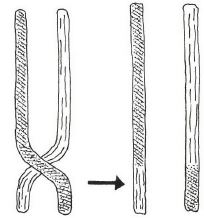
\includegraphics[width=0.2\textwidth]{./img/vso/cross-over.jpg}
\end{center}

\begin{description*}
%\item[Subtopic:]{}
\item[Materials:]{Manila paper, cotton swabs, tape, string, markers}
%\item[Setup:]{}
\item[Procedure:]{Construct models of the different stages of meiosis using cotton swabs or toothpicks. Overlap two and tape together to show crossing over.}
%\item[Hazards:]{}
%\item[Questions:]{}
%\item[Observations:]{}
\item[Theory:]{In
meiosis pairs of chromosomes
come to lie next to each other. At
points called chiasmata, parts of
chromosomes are exchanged. This
crossing over results in exchange
of genes.}
%\item[Applications:]{}
%\item[Notes:]{}
\end{description*}

%\subsection{Crossing Over} % VSO 53
%
%\begin{center}
%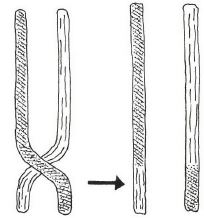
\includegraphics[width=0.2\textwidth]{./img/vso/cross-over.jpg}
%\end{center}
%
%\begin{description*}
%%\item[Subtopic:]{}
%\item[Materials:]{Clay/Plasticine}
%%\item[Setup:]{}
%\item[Procedure:]{Make 2 chromosomes of different
%colours in clay or Plasticine. }
%%\item[Hazards:]{}
%%\item[Questions:]{}
%%\item[Observations:]{}
%\item[Theory:]{In
%meiosis pairs of chromosomes
%come to lie next to each other. At
%points called chiasmata, parts of
%chromosomes are exchanged. This
%crossing over results in exchange
%of genes.}
%%\item[Applications:]{}
%%\item[Notes:]{}
%\end{description*}

%==================================================================================================%

\section*{Reproduction in Flowering \hfill \\  Plants}


\subsection{Flower Structure} % VSO 51

\begin{center}
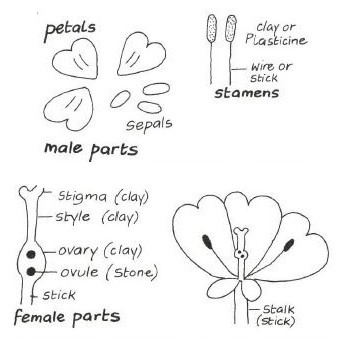
\includegraphics[width=0.4\textwidth]{./img/vso/flower-structure.jpg}
\end{center}

\begin{description*}
%\item[Subtopic:]{}
\item[Materials:]{Card or plastic, sticks, stones paper, clay or Plasticine}
%\item[Setup:]{}
\item[Procedure:]{Make the major parts of a flower from card or plastic, sticks and clay.
Petals can be made from paper.}
%\item[Hazards:]{}
%\item[Questions:]{}
%\item[Observations:]{}
%\item[Theory:]{}
\item[Applications:]{Look at a variety of flowers, fruit and seeds from the local environment.}
%\item[Notes:]{}
\end{description*}

\columnbreak

\subsection{Anthers and Pollen}

\begin{center}
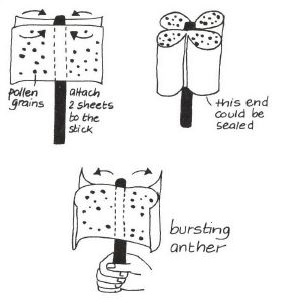
\includegraphics[width=0.4\textwidth]{./img/vso/anthers-pollen.jpg}
\end{center}

\begin{description*}
%\item[Subtopic:]{}
\item[Materials:]{Paper, sticks}
%\item[Setup:]{}
\item[Procedure:]{Make a model of an anther as shown. Lightly glue small pieces of card
or stick onto paper to represent pollen. Alternatively draw circles to
represent the pollen. }
%\item[Hazards:]{}
%\item[Questions:]{}
%\item[Observations:]{}
\item[Theory:]{When the paper is folded it represents anthers
full of pollen. They are ready to burst open and shed pollen into the
wind or onto insects.}
\item[Applications:]{Look at a variety of flowers, fruit and seeds from the local environment.}
%\item[Notes:]{}
\end{description*}

%==================================================================================================%

\section*{Reproduction in Mammals}


\subsection{Sperm and Egg} % VSO 50

\begin{center}
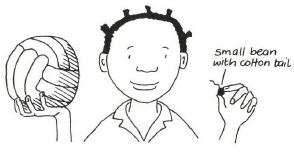
\includegraphics[width=0.4\textwidth]{./img/vso/sperm-egg.jpg}
\end{center}

\begin{description*}
%\item[Subtopic:]{}
\item[Materials:]{Football, bean}
%\item[Setup:]{}
%\item[Procedure:]{}
%\item[Hazards:]{}
%\item[Questions:]{}
%\item[Observations:]{}
\item[Theory:]{The football represents the
human egg, the bean a human
sperm}
%\item[Applications:]{}
%\item[Notes:]{}
\end{description*}

\columnbreak

\subsection{Sperm Model}

\begin{center}
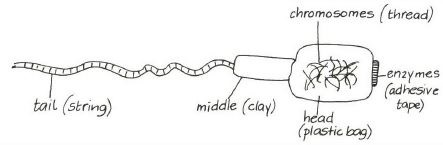
\includegraphics[width=0.49\textwidth]{./img/vso/sperm-model.jpg}
\end{center}

\begin{description*}
%\item[Subtopic:]{}
\item[Materials:]{Plastic bag, tape, string, thread/steel wool, clay}
%\item[Setup:]{}
\item[Procedure:]{Construct a simple sperm model as shown.}
%\item[Hazards:]{}
%\item[Questions:]{}
%\item[Observations:]{}
%\item[Theory:]{}
%\item[Applications:]{}
%\item[Notes:]{}
\end{description*}

\subsection{Amniotic Sac Protection}

\begin{center}
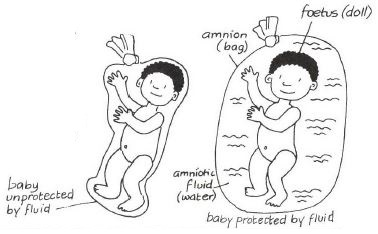
\includegraphics[width=0.49\textwidth]{./img/vso/amniotic-sac.jpg}
\end{center}

\begin{description*}
%\item[Subtopic:]{}
\item[Materials:]{Doll, clear plastic bag, water}
%\item[Setup:]{}
\item[Procedure:]{Place a plastic doll into an empty,
clear plastic bag. Fill the plastic
bag with water, place the doll
inside and knot the opening so it
is sealed. Pass the water-filled bag
around and discuss with students
what protects a baby inside the
mother.}
%\item[Hazards:]{}
%\item[Questions:]{}
%\item[Observations:]{}
%\item[Theory:]{}
%\item[Applications:]{}
%\item[Notes:]{}
\end{description*}

\columnbreak

\subsection{Fertilisation}

\begin{center}
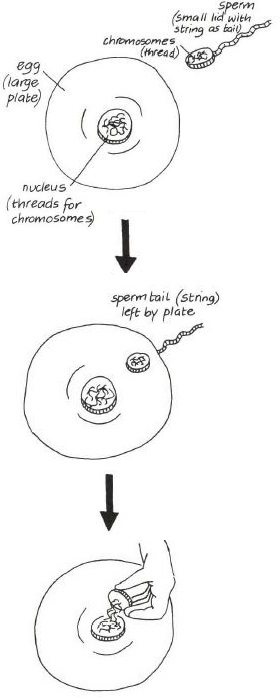
\includegraphics[width=0.45\textwidth]{./img/vso/fertilisation.jpg}
\end{center}

\begin{description*}
%\item[Subtopic:]{}
\item[Materials:]{2 bottle lids, thread, string, large plate}
%\item[Setup:]{}
\item[Procedure:]{Make the sperm and egg cell as shown. Note that the lids represent the
nuclei of the female and male cells. The plate represents the egg cell.
The fine threads represent chromosomes. Move the sperm towards the
egg cell until it touches the nucleus of the egg cell. Mix the threads
from both lids. This represents the sperm head bursting and the mixing
of chromosomes.}
%\item[Hazards:]{}
%\item[Questions:]{}
%\item[Observations:]{}
%\item[Theory:]{}
%\item[Applications:]{}
%\item[Notes:]{}
\end{description*}


\end{multicols}

\pagebreak